\newpage
\subsection{Importing and working with multiple EAPs}
\visHeader
\label{sec:multiEAP}

It should be mentioned here that the following instructions are about how to properly export and import EA files. You may want to bookmark this section so that
you can reference it later for your own projects. It should be noted that we could have easily shortened this process and just provided the import file as a
download, but we want to stress the importance of how to properly import and extract EAP projects.

\begin{itemize}

\item[$\blacktriangleright$] In the same \texttt{Part4.zip} folder you extracted this document from, open the \texttt{DictionaryLanguageSource.eap} file in
Enterprise Architect (EA). % Rearrange this so the definition is in the paragraph above? (ie: eap == enterprise architect project)

\item[$\blacktriangleright$] The expanded rootnote should look like Fig.~\ref{fig:dictionaryLangStart}. Please note that while you could simply copy and paste
single packages between multiple EAPs (i.e., copy \texttt{<<EPackage>>DictionaryLanguage} into the \texttt{MyWorkingSet} root note)(\update test this), if there
are packages with dependencies on other packages, it cannot be copied so easily. If you did this, all links would be destroyed!

\begin{figure}[htbp]
\begin{center}
  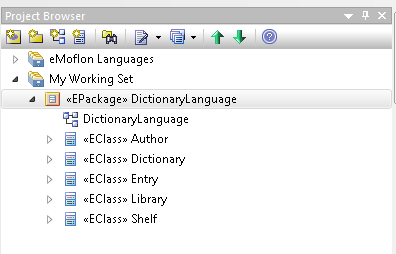
\includegraphics[width=0.5\textwidth]{ea_dictLangProBrowser}
  \caption{caption}
  \label{fig:dictionaryLangStart}
\end{center}
\end{figure}

\item[$\blacktriangleright$] Therefore, to migrate multiple pacakges, you have to first export a \emph{complete} root node to an XMI file. First right-click on
the root \texttt{DictionaryLanguage}, then navigate to ``Export Model to XMI\ldots'' (Fig.~\ref{fig:contextExport}). Alternatively, select the root and press
\texttt{Ctrl + Alt + E}.

\begin{figure}[htbp]
\begin{center}
  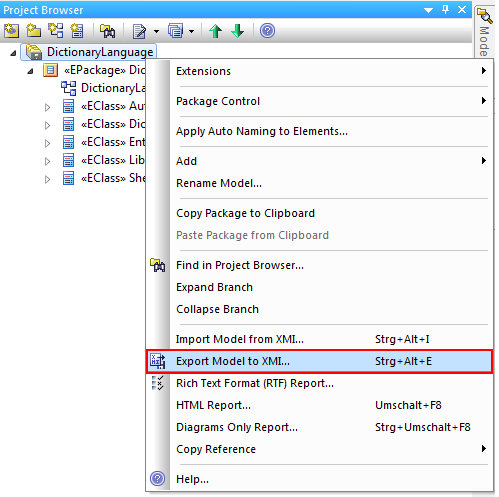
\includegraphics[width=0.7\textwidth]{ea_exportToXMI}
  \caption{caption}
  \label{fig:contextExport}
\end{center}
\end{figure}

\item[$\blacktriangleright$] Save the file somewhere easily accessible, such as your desktop, and change the export type to \texttt{XMI 2.1}. Press export,
and close the window once the small green bar appears (Fig.~\ref{fig:exportDialogue}).

\vspace{0.5cm}

\begin{figure}[htbp]
\begin{center}
  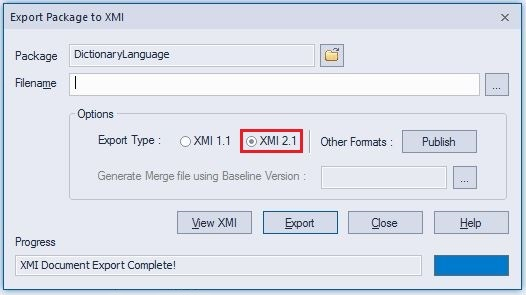
\includegraphics[width=0.8\textwidth]{ea_dialogueExport}
  \caption{caption}
  \label{fig:export}
\end{center}
\end{figure}

\item[$\blacktriangleright$] Now re-open \texttt{LeitnersLearningBox.eap} from Eclipse and right-click anywhere in the project browser. Navigate to ``Import
Model from XMI\ldots''

\item[$\blacktriangleright$] Find the \texttt{.xmi} file you just saved and press \texttt{import}. Press \texttt{OK} in the confirmation dialogue. You workspace
should now resemble Fig. \update
% Fig.~\ref{}

\item[$\blacktriangleright$] The final step is to \texttt{Validate All}\footnote{To review how to use the eMoflon control panel, read Part II Section 2.8} and
refresh your Eclipse workspace. Two newly generated projects should appear in your working set, \texttt{Dictionary Adapter} and \texttt{Dictionary Language}. 

\item[$\blacktriangleright$] If you've just joined us and are interested in the eMoflon project structure, and are curious as to how metamodels and generated
code are related, we invite you to read Part I, Section 4.1. Otherwise, you're read to begin working with TGGs! 

\jumpSingle{TGGSchema}

\end{itemize}
